\documentclass[conference]{IEEEtran}
\IEEEoverridecommandlockouts
\usepackage{cite}
\usepackage{amsmath,amssymb,amsfonts}
\usepackage{algorithmic}
\usepackage{graphicx}
\usepackage{textcomp}
\usepackage{xcolor}
\usepackage{array}
\usepackage{tikz}
\usetikzlibrary{arrows.meta}
\definecolor{fbNavy}{HTML}{1F3A5F}
\definecolor{fbGray}{HTML}{7A7A7A}
\definecolor{fbPurple}{HTML}{6A3D9A}
\definecolor{fbGreen}{HTML}{6B8E23}
\definecolor{fbOrange}{HTML}{E07B39}
\definecolor{fbTeal}{HTML}{2A7F8E}
\definecolor{fbBlue}{HTML}{A6D8E6}
\definecolor{fbRed}{HTML}{B03A2E}
\def\BibTeX{{\rm B\kern-.05em{\sc i\kern-.025em b}\kern-.08em
    T\kern-.1667em\lower.7ex\hbox{E}\kern-.125emX}}
\setlength{\textfloatsep}{8pt plus 2pt minus 2pt}
\setlength{\floatsep}{6pt plus 2pt minus 2pt}
\begin{document}

\title{Evaluating Large Language Models on Multi-Step Discounted Cash Flow Valuation}

\author{\IEEEauthorblockN{Hawon Kim}
\IEEEauthorblockA{\textit{Department of Operations and} \\
\textit{Decision Technologies} \\
\textit{Indiana University}\\
Bloomington, IN, USA \\
hawkim@iu.edu}
\and
\IEEEauthorblockN{Jianna Hur}
\IEEEauthorblockA{\textit{Department of Operations and} \\
\textit{Decision Technologies} \\
\textit{Indiana University}\\
Bloomington, IN, USA \\
jhur06@iu.edu}
\and
\IEEEauthorblockN{Sagar Samtani}
\IEEEauthorblockA{\textit{Department of Operations and} \\
\textit{Decision Technologies} \\
\textit{Indiana University}\\
Bloomington, IN, USA \\
ssamtani@iu.edu}
}

\maketitle

\begin{abstract}
Discounted cash flow (DCF) valuation is one of the most widely used methods for estimating firm value, and large language models (LLMs) are increasingly applied to this kind of financial analyst work. However, there is limited evidence on how LLMs perform on multi-step financial workflows. A DCF is a chain of dependent steps, so an early mistake carries through to the value per share without any sign of where it started, and a benchmark that scores only the final number cannot locate the failure. In this study, we propose a staged DCF benchmark of 308 questions on 33 U.S. public companies at three valuation dates, in which every intermediate checkpoint is graded against a deterministic answer key. We evaluate twelve open-weight LLMs, six of them financial fine-tunes, and find that accuracy falls with workflow length for every model. Qwen2.5-32B answers 80\% of single calculations but no full DCF under the textbook policy, and only the reasoning models complete full valuations. Neither financial fine-tuning nor a calculator substitutes for a reasoning mode, and the remaining errors of the best model arise mostly from omitted conventions and from small numerical deviations that later steps magnify.
\end{abstract}

\begin{IEEEkeywords}
large language models, financial reasoning, discounted cash flow, valuation, benchmark, human-in-the-loop
\end{IEEEkeywords}


\section{Introduction}\label{sec:intro}
Company valuation is central to many financial decisions, such as whether to buy or sell a stock, how much to offer in a merger, and whether a project should be funded. Among valuation methods, the discounted cash flow (DCF) model is the most widely used. About four in five finance practitioners report using DCF models for valuation \cite{b1}, and practitioner surveys rank DCF with market multiples as the most common technique \cite{b2}. DCF has remained in use because it derives value from the firm's own forecast cash flows and cost of capital and records every assumption where it can be examined \cite{b3}. It is also a multi-step workflow in which each step depends on the output of the previous one, so the final value per share is only as reliable as the steps that precede it.

\begin{figure}[!t]
\centering
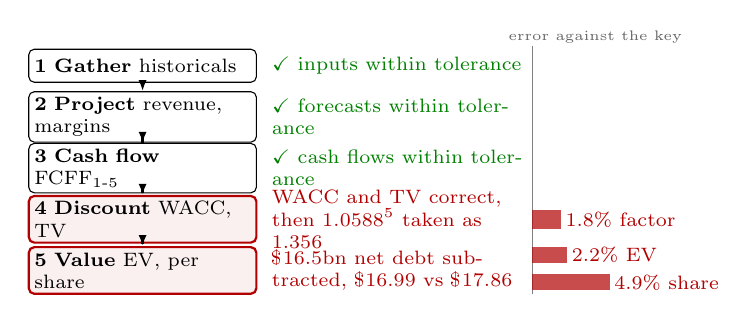
\begin{tikzpicture}[x=1cm,y=1cm, font=\scriptsize,
  box/.style={draw, rounded corners=2pt, align=left, minimum height=0.42cm, text width=2.75cm, inner sep=2pt},
  hot/.style={box, draw=red!70!black, thick, fill=red!70!black, fill opacity=0.06, text opacity=1},
  flow/.style={-{Latex[length=1.4mm]}, thick},
  note/.style={align=left, inner sep=1pt, text width=3.25cm}]
\node[box] (s1) at (0,2.6) {\textbf{1 Gather} historicals};
\node[box] (s2) at (0,1.95) {\textbf{2 Project} revenue, margins};
\node[box] (s3) at (0,1.3) {\textbf{3 Cash flow} FCFF$_{1\text{-}5}$};
\node[hot] (s4) at (0,0.65) {\textbf{4 Discount} WACC, TV};
\node[hot] (s5) at (0,0.0) {\textbf{5 Value} EV, per share};
\draw[flow] (s1) -- (s2); \draw[flow] (s2) -- (s3); \draw[flow] (s3) -- (s4); \draw[flow] (s4) -- (s5);
\node[note, green!50!black, anchor=west] at (1.6,2.6) {$\checkmark$ inputs within tolerance};
\node[note, green!50!black, anchor=west] at (1.6,1.95) {$\checkmark$ forecasts within tolerance};
\node[note, green!50!black, anchor=west] at (1.6,1.3) {$\checkmark$ cash flows within tolerance};
\node[note, red!70!black, anchor=west] at (1.6,0.65) {WACC and TV correct, then $1.0588^5$ taken as 1.356};
\node[note, red!70!black, anchor=west] at (1.6,0.0) {\$16.5bn net debt subtracted, \$16.99 vs \$17.86};
% error bars, 0.2 cm per percentage point
\draw[black!50] (4.95,-0.3) -- (4.95,2.85);
\node[anchor=south, inner sep=1pt, black!60, font=\tiny] at (5.75,2.85) {error against the key};
\fill[red!70!black, fill opacity=0.7] (4.95,0.53) rectangle (5.31,0.77);
\node[anchor=west, inner sep=1pt, red!70!black] at (5.33,0.65) {1.8\% factor};
\fill[red!70!black, fill opacity=0.7] (4.95,0.1) rectangle (5.39,0.3);
\node[anchor=west, inner sep=1pt, red!70!black] at (5.41,0.2) {2.2\% EV};
\fill[red!70!black, fill opacity=0.7] (4.95,-0.25) rectangle (5.93,-0.05);
\node[anchor=west, inner sep=1pt, red!70!black] at (5.95,-0.15) {4.9\% share};
\end{tikzpicture}
\caption{Error propagation in a DCF valuation of PPL Corporation.}
\label{fig:chain}
\end{figure}

Large language models (LLMs) are increasingly applied to this kind of multi-step analyst work. LLMs read news and filings at scale, GPT-4 predicts the direction of market reactions to headlines without financial training \cite{b4}, and commercial assistants draft financial models from filings. In these applications, the model mainly reads and retrieves information, while the calculations and decisions at each step remain with the analyst. This division reflects known limits, as LLM accuracy on adding balance-sheet items declines toward zero as the number of items increases, and a DuPont analysis from full financial statements is correct only 30 to 40 percent of the time \cite{b5}. Whether a model can be trusted with a complete valuation therefore depends on where along the workflow its errors arise, which is a question about individual steps rather than about the final number.

Existing financial benchmarks, however, cannot show where along a valuation a model fails. Question-answering datasets require only a few operations over a table or a passage \cite{b6,b7,b8,b9}. More recent benchmarks extend to professional workflows in finance \cite{b10,b11,b12}, but they grade these workflows with rubric items judged by another LLM, and none holds a single workflow fixed while varying its length or components. As a result, an error cannot be traced to the step at which it occurred, although that step is where an analyst would intervene.

Building a benchmark that can locate these failures poses three difficulties. First, a DCF is a long chain of dependent steps (Fig.~\ref{fig:chain}), and an early error is carried to the end and often magnified. In Fig.~\ref{fig:chain}, a reasoning model computed every input and cash flow, the weighted average cost of capital (WACC) and the terminal value (TV) within tolerance, but took 1.0588 to the fifth power as 1.356 instead of 1.331. The resulting 1.8 percent error in the year-5 discount factor became 2.2 percent in enterprise value (EV) and, after about 16.5 billion dollars of net debt was subtracted, 4.9 percent in the value per share. Second, a DCF has no single correct answer. The risk-free rate, the equity risk premium, the beta adjustment, the terminal growth rate and the timing of discounting are judgment calls on which textbooks and practitioners differ \cite{b3}, and even the definition of cash flow can change conclusions \cite{b13}, so an answer key exists only when these choices are stated. Third, the companies are publicly traded and their filings may be in training data, so scoring against observed market values would reward recall rather than valuation skill \cite{b5,b14}.

To address these difficulties, we introduce a staged DCF benchmark.\footnote{The questions, answer keys and grading code are available at \texttt{https://github.com/[placeholder]}.} Its purpose is to show whether an LLM can complete a valuation and, if not, at which step it fails, so that an analyst knows where to review. The benchmark has three components.
\begin{enumerate}
\item A staged task design that presents the same companies at several workflow lengths, from a single calculation through two complementary half-workflows to a complete valuation, so that the effect of the chain is isolated.
\item A policy-specified answer key that states every judgment call in the question, so that a deterministic engine computes a single answer at every step that cannot be recalled from market prices.
\item A step-level grading scheme that scores each checkpoint against that key, adds trap questions with a tempting incorrect figure, and measures the chain gap, the failures that arise only when correctly solved parts are combined.
\end{enumerate}
We apply the benchmark to twelve open-weight LLMs, six of them financial fine-tunes, on 308 questions spanning 33 U.S. public companies and three valuation dates.

\section{Related Work}\label{sec:related}
We first review past research relevant to the three difficulties of Section~\ref{sec:intro} (Sections~\ref{sec:rwA} to~\ref{sec:rwC}) and then the financial benchmarks closest to our setting (Section~\ref{sec:rwD}).

\subsection{Compositional Failures in Multi-Step Reasoning}\label{sec:rwA}
Models often answer every sub-question of a composed question correctly but fail the composed question itself, and this compositionality gap does not decrease even as models grow larger \cite{b15}. Checking every reasoning step is more effective than checking only the final answer \cite{b16}, and ProcessBench asks models to locate the earliest incorrect step in a mathematical solution \cite{b17}. Both rely on human step labels, whereas P2S derives step rewards from a model's own probabilities \cite{p2s}. In a DCF with stated conventions, an engine supplies the correct value of every step, so the compositionality gap can be measured directly as the chain gap of Section~\ref{sec:tiers}.

\subsection{Judgment Calls in DCF Valuation}\label{sec:rwB}
The DCF procedure itself is standard. As Figs.~\ref{fig:chain} and~\ref{fig:framework} show, an analyst forecasts free cash flows, discounts them at the WACC, adds a terminal value and bridges from enterprise value to a value per share \cite{b3}. The inputs to these steps, however, are judgment calls on which textbooks and practitioners differ \cite{b3}, and even the definition of cash flow changes the conclusions of published studies \cite{b13}. For PPL Corporation, the textbook and practitioner policies of Section~\ref{sec:policy} give \$17.86 and \$20.43 per share from the same filings. A benchmark therefore has to state every judgment call in the question before it can define a correct answer.

\subsection{Numerical Limits and Look-Ahead Bias of LLMs}\label{sec:rwC}
Even with the conventions stated, two properties of LLMs complicate evaluation. First, their accuracy on financial arithmetic declines as the number of inputs grows and approaches 100 percent only when the model writes code that an interpreter executes \cite{b5}, so a valuation benchmark should separate arithmetic errors from reasoning errors. Second, their predictions may reflect memorized outcomes, as GPT-4's earnings-prediction accuracy falls to chance when only the last digit of each input is randomized \cite{b5}. Chronologically consistent models are trained on time-restricted data to remove this leakage \cite{b14}, and a benchmark should likewise score answers against values that cannot be memorized.

\subsection{Step-Level Grading in Financial Benchmarks}\label{sec:rwD}
Existing financial benchmarks address parts of these problems. FinQA, TAT-QA and ConvFinQA pose numerical questions over financial tables and text with exact answers, but each answer requires only a few operations \cite{b6,b7,b8}, and FinBen combines many such datasets \cite{b9}. BigFinanceBench, MBABench and HERCULEAN extend evaluation to analyst workflows such as DCF and leveraged buyout models, and all three find that agents weaken as tasks require more chained calculations \cite{b10,b11,b12}.

\section{Research Gaps and Questions}\label{sec:rq}
Prior research in Section~\ref{sec:related} leaves three limitations. First, financial benchmarks of analyst workflows fix the length of each task, so it is not known how accuracy changes when the same valuation becomes longer. Second, step-level evaluation has been applied mostly to mathematical problems with labeled steps, and workflow benchmarks rely on LLM judges, so it remains unclear at which steps of a valuation errors arise. Third, the numerical limits of LLMs have been examined on single calculations, so it is unclear whether scale, a reasoning mode, financial fine-tuning or a calculator overcomes them in a chained valuation. Accordingly, each limitation leads to one of the following research questions.
\begin{list}{}{\setlength{\leftmargin}{2.5em}\setlength{\labelwidth}{2.1em}\setlength{\labelsep}{0.4em}\setlength{\itemsep}{0pt}\setlength{\parsep}{0pt}\setlength{\topsep}{3pt}}
\item[RQ1.] How does accuracy change from a single calculation to a full DCF valuation?
\item[RQ2.] At which steps do errors arise, and of what kind?
\item[RQ3.] Do model scale, a reasoning mode, financial fine-tuning or a calculator improve accuracy on long valuations?
\end{list}

\section{Research Design}\label{sec:design}
\begin{figure*}[t]
\centering
\resizebox{\textwidth}{!}{%
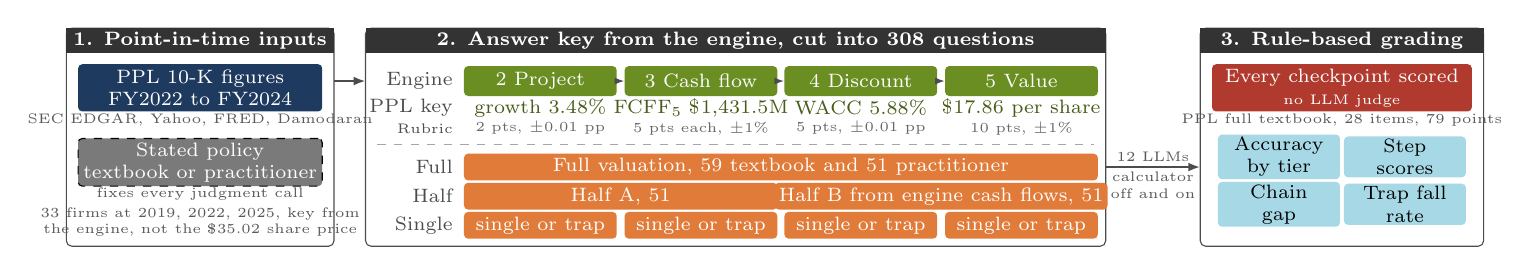
\begin{tikzpicture}[x=1cm,y=0.86cm, font=\scriptsize,
  panel/.style={draw=black!70, rounded corners=2pt},
  band/.style={text=white, font=\scriptsize\bfseries, inner sep=0pt},
  box/.style={rounded corners=1.5pt, align=center, inner sep=1.5pt},
  stp/.style={box, fill=fbGreen, text=white, minimum width=1.94cm, minimum height=0.38cm},
  tier/.style={box, fill=fbOrange, text=white, minimum height=0.34cm},
  met/.style={box, fill=fbBlue, text=black, text width=1.45cm, minimum width=1.55cm, minimum height=0.46cm, inner sep=1pt},
  key/.style={text=fbGreen!65!black, inner sep=0pt},
  pts/.style={font=\tiny, text=black!60, inner sep=0pt},
  lab/.style={anchor=east, inner sep=1pt, text=black!70},
  note/.style={font=\tiny, text=black!65, align=center, inner sep=0pt},
  arr/.style={-{Latex[length=1.5mm]}, thick, black!70}]
% ---------- panels ----------
\draw[panel] (0,0.38) rectangle (3.4,3.6);        \fill[black!80] (0,3.24) rectangle (3.4,3.6);
\node[band] at (1.7,3.42) {1. Point-in-time inputs};
\draw[panel] (3.8,0.38) rectangle (13.2,3.6);     \fill[black!80] (3.8,3.24) rectangle (13.2,3.6);
\node[band] at (8.5,3.42) {2. Answer key from the engine, cut into 308 questions};
\draw[panel] (14.4,0.38) rectangle (18.0,3.6);    \fill[black!80] (14.4,3.24) rectangle (18.0,3.6);
\node[band] at (16.2,3.42) {3. Rule-based grading};
% ---------- 1. inputs ----------
\node[box, fill=fbNavy, text=white, minimum width=3.1cm, minimum height=0.6cm] at (1.7,2.72) {PPL 10-K figures\\FY2022 to FY2024};
\node[note] at (1.7,2.25) {SEC EDGAR, Yahoo, FRED, Damodaran};
\node[box, fill=fbGray, text=white, draw=black, dashed, minimum width=3.1cm, minimum height=0.6cm] at (1.7,1.62) {Stated policy\\textbook or practitioner};
\node[note] at (1.7,1.15) {fixes every judgment call};
\node[note] at (1.7,0.74) {33 firms at 2019, 2022, 2025, key from\\the engine, not the \$35.02 share price};
\draw[arr] (3.4,2.82) -- (3.8,2.82);
% ---------- 2. engine checkpoints (step columns at 6.02, 8.06, 10.09, 12.13) ----------
\node[lab] at (4.95,2.82) {Engine};
\node[stp] (e2) at (6.02,2.82) {2 Project};
\node[stp] (e3) at (8.06,2.82) {3 Cash flow};
\node[stp] (e4) at (10.09,2.82) {4 Discount};
\node[stp] (e5) at (12.13,2.82) {5 Value};
\foreach \a/\b in {e2/e3,e3/e4,e4/e5} \draw[-{Latex[length=1.2mm]}, black!70] (\a) -- (\b);
\node[lab] at (4.95,2.42) {PPL key};
\node[key] at (6.02,2.42) {growth 3.48\%};
\node[key] at (8.06,2.42) {FCFF$_5$ \$1,431.5M};
\node[key] at (10.09,2.42) {WACC 5.88\%};
\node[key] at (12.13,2.42) {\$17.86 per share};
\node[lab, font=\tiny] at (4.95,2.12) {Rubric};
\node[pts] at (6.02,2.12) {2 pts, $\pm$0.01 pp};
\node[pts] at (8.06,2.12) {5 pts each, $\pm$1\%};
\node[pts] at (10.09,2.12) {5 pts, $\pm$0.01 pp};
\node[pts] at (12.13,2.12) {10 pts, $\pm$1\%};
\draw[black!35, dashed] (3.95,1.88) -- (13.05,1.88);
% ---------- 2. tiers under the steps they cover ----------
\node[lab] at (4.95,1.55) {Full};
\node[tier, minimum width=8.05cm] at (9.075,1.55) {Full valuation, 59 textbook and 51 practitioner};
\node[lab] at (4.95,1.12) {Half};
\node[tier, minimum width=3.98cm] at (7.04,1.12) {Half A, 51};
\node[tier, minimum width=3.98cm] at (11.11,1.12) {Half B from engine cash flows, 51};
\node[lab] at (4.95,0.69) {Single};
\foreach \x in {6.02,8.06,10.09,12.13} \node[tier, minimum width=1.94cm] at (\x,0.69) {single or trap};
% ---------- hand-off to grading ----------
\draw[arr] (13.2,1.55) -- (14.4,1.55);
\node[note, anchor=south] at (13.8,1.62) {12 LLMs};
\node[note, anchor=north] at (13.8,1.48) {calculator\\off and on};
% ---------- 3. grading ----------
\node[box, fill=fbRed, text=white, minimum width=3.3cm, minimum height=0.6cm] at (16.2,2.72) {Every checkpoint scored\\{\tiny no LLM judge}};
\node[note] at (16.2,2.25) {PPL full textbook, 28 items, 79 points};
\node[met] at (15.4,1.7) {Accuracy\\by tier};
\node[met] at (17.0,1.7) {Step\\scores};
\node[met] at (15.4,1.0) {Chain\\gap};
\node[met] at (17.0,1.0) {Trap fall\\rate};
\end{tikzpicture}}
\caption{Benchmark design traced for PPL Corporation at 2025-12-31.}
\label{fig:framework}
\end{figure*}

To answer these questions, we built the benchmark in Fig.~\ref{fig:framework}, traced for PPL Corporation from the inputs (Section~\ref{sec:data}) through the answer key and tiers (\ref{sec:policy}, \ref{sec:tiers}) to the model runs and grading (\ref{sec:models}, \ref{sec:grading}).

\subsection{Point-in-Time Company Data}\label{sec:data}
We build every question from a snapshot frozen at its valuation date, so that it can be regenerated exactly and contains no data published after that date. Financial statement items come from SEC EDGAR XBRL data\footnote{SEC is the U.S. Securities and Exchange Commission, EDGAR its Electronic Data Gathering, Analysis, and Retrieval system, XBRL the eXtensible Business Reporting Language, FRED the Federal Reserve Economic Data service, and GICS the Global Industry Classification Standard.} for 10-K filings made on or before the valuation date, share prices from Yahoo Finance, Treasury rates from FRED, and industry betas and default spreads from Damodaran \cite{b3}. The main set contains the 28 largest U.S.-listed non-financial 10-K filers across eight GICS sectors with a December fiscal year-end and positive earnings before interest and taxes (EBIT) and free cash flow to the firm (FCFF) in each of the three prior years, valued as of December 31, 2025. To separate the rate environment from the firm, 13 of these firms are also valued as of December 31, 2019 and 2022, and five held-out firms are added at 2025 (Table~\ref{tab:data}). The answer key is the engine's value rather than the observed price (\$17.86 against \$35.02 for PPL), so it cannot be recalled.

\subsection{Valuation Policies and Answer Engine}\label{sec:policy}
Each question states a valuation policy that fixes every judgment call, so that a single answer exists. The textbook policy follows standard corporate finance conventions \cite{b18}, and the practitioner policy changes seven of its rules (the 10-year yield instead of the 3-month bill, a 5.0\% \cite{b19} instead of a 7.0\% equity risk premium, a Blume-adjusted beta \cite{b20}, effective instead of statutory tax in years 1 to 4, mid-year instead of year-end discounting, 2.5\% instead of 2.0\% terminal growth, and an operating cash reserve of 2\% of revenue instead of treating all cash as excess).

Under the stated policy, a deterministic engine computes the answer through the five steps of Fig.~\ref{fig:chain} and stores every intermediate value as a checkpoint. Step 2 grows revenue from its three-year growth rate toward the terminal rate $g$ and holds the other items at their average shares of revenue. Step 3 computes FCFF as after-tax EBIT plus depreciation and amortization, less capital expenditures and the change in net working capital, with year 5 in a steady state. Step 4 estimates the cost of equity with the capital asset pricing model (CAPM) and the cost of debt as the 10-year yield plus the rating spread, and discounts at the WACC with \mbox{$\mathit{TV} = \mathit{FCFF}_5(1+g)/(\mathit{WACC}-g)$}. Step 5 bridges to equity value and divides by diluted shares. The engine reproduces a published textbook example to the cent \cite{b18}, and an independent re-implementation matched every target within 0.032\%.

\begin{table}[t]
\caption{QUESTIONS BY VALUATION SET AND TIER (TB, TEXTBOOK POLICY, PR, PRACTITIONER POLICY)}
\centering
\scriptsize
\renewcommand{\arraystretch}{0.9}
\setlength{\tabcolsep}{3pt}
\begin{tabular}{|l|r|r|r|r|r|r|r|}
\hline
\textbf{Set (firms)} & \textbf{Single} & \textbf{Trap} & \textbf{Half A} & \textbf{Half B} & \textbf{Full TB} & \textbf{Full PR} & \textbf{Total} \\ \hline
2025 (28) & 56 & 40 & 20 & 20 & 28 & 20 & 184 \\
2019 (13) & & & 13 & 13 & 13 & 13 & 52 \\
2022 (13) & & & 13 & 13 & 13 & 13 & 52 \\
Held-out (5) & & & 5 & 5 & 5 & 5 & 20 \\ \hline
Total (33) & 56 & 40 & 51 & 51 & 59 & 51 & 308 \\ \hline
\end{tabular}
\label{tab:data}
\end{table}

\subsection{Staged Question Tiers}\label{sec:tiers}
We cut 308 questions from these checkpoints at four workflow lengths, so that for the same company only the length of the task changes (Table~\ref{tab:data} and Fig.~\ref{fig:framework}). Single-step questions ask for one calculation, such as the cost of equity of PPL, and trap questions also present the figure that one of twelve common DCF errors would produce. For PPL, the rule states that the cost of debt is the 10-year yield plus the rating spread, while the question also reports interest expense, whose ratio to debt gives a WACC of 5.52\% instead of 5.88\%. Half A ends at the five free cash flows and Half B starts from the engine's cash flows, so an error in one half cannot enter the other. Because the two halves compose exactly to the full textbook valuation, a company whose halves are both correct but whose full valuation is wrong has failed only in combining them, which we call the chain gap. Every question prints its policy and the historical figures it needs, so Step 1 is supplied rather than tested.

\subsection{Models and Inference Settings}\label{sec:models}
We compare twelve open-weight models in pairs that differ in one property. Scale varies within Qwen2.5 (7B and 32B Instruct \cite{b21}) and the reasoning mode within Qwen3 (8B, 14B and 32B in thinking mode \cite{b22}), and Llama-3.1-8B-Instruct \cite{b23} adds a second model family. Six financial fine-tunes, Fin-R1 \cite{b24}, DianJin-R1-7B and 32B \cite{b25}, Fin-o1-8B and 14B and Fino1-8B \cite{b26}, are each compared with their base model (Table~\ref{tab3}). Each model answers every question with and without a calculator tool (up to 300 calls per answer) to separate arithmetic errors from reasoning errors. Reasoning models are sampled at their recommended settings under three seeds with up to 24,576 new tokens, the other models decode greedily once with up to 8,192, and only the response after the reasoning trace is graded.

\subsection{Rubric-Based Grading and Metrics}\label{sec:grading}
We grade every checkpoint with a deterministic rubric instead of an LLM judge. Each question has one rubric item per checkpoint it covers, with the points in Fig.~\ref{fig:framework}. Rates must match within 0.01 percentage points (pp) and dollar values within 1\%. The grader reads the final answer after the last answer marker the model used, such as \verb|\boxed{}|, because the financial fine-tunes rarely produce the requested line. We report final-answer accuracy by tier pooled over seeds, step scores as the share of rubric points earned within each step, the chain gap, and the trap fall rate, the share of trap answers that match the trap figure.

\section{Results}
\begin{table}[t]
\caption{ACCURACY (\%) WITHOUT AND WITH (+C) THE CALCULATOR}
\centering
\scriptsize
\renewcommand{\arraystretch}{0.82}
\begin{tabular}{|l|r|r|r|r|}
\hline
\textbf{Model (base)} & \textbf{Single} & \textbf{Full, textbook} & \textbf{All} & \textbf{All, +C} \\ \hline
Qwen2.5-7B-Instruct & 78.6 & 0.0 & 25.6 & 26.3 \\
Qwen2.5-32B-Instruct & 80.4 & 0.0 & 34.4 & 56.5 \\
Llama-3.1-8B-Instruct & 33.9 & 0.0 & 9.7 & 12.3 \\
Qwen3-8B, thinking & 90.5 & 15.5 & 66.9 & 70.2 \\
Qwen3-14B, thinking & 97.6 & 33.3 & 75.6 & 71.5 \\
Qwen3-32B, thinking & 89.3 & 85.7 & 91.7 & 79.0 \\ \hline
Fin-R1 (Qwen2.5-7B) & 60.1 & 2.4 & 21.2 & 18.9 \\
DianJin-R1-7B (Qwen2.5-7B) & 88.1 & 0.0 & 30.5 & 31.7 \\
DianJin-R1-32B (Qwen2.5-32B) & 97.6 & 16.7 & 66.8 & 61.4 \\
Fin-o1-8B (Qwen3-8B) & 58.3 & 1.2 & 21.4 & 22.5 \\
Fin-o1-14B (Qwen3-14B) & 69.6 & 3.6 & 25.2 & 25.0 \\
Fino1-8B (Llama-3.1-8B) & 28.6 & 0.0 & 10.0 & 10.0 \\ \hline
\end{tabular}
\label{tab3}
\end{table}

\subsection{Accuracy Declines as the Workflow Lengthens (RQ1)}
Accuracy falls with workflow length for every model (Table~\ref{tab3}). Qwen2.5-32B answers 80\% of single calculations but no full textbook valuation, DianJin-R1-32B and Qwen3-14B fall from 98\% to 17\% and 33\%, and Qwen3-32B keeps 86\%. The chain gap shows that the decline comes from combining steps, as DianJin-R1-32B, Qwen3-8B and Qwen3-14B failed the full valuation in 93\%, 91\% and 71\% of the company-seed pairs with both halves correct, against 20\% for Qwen3-32B. Neither the date nor the policy explains the decline, as Qwen3-32B's full textbook accuracy is 87 to 95\% on the other sets and the practitioner policy was no harder on the same firms.

\subsection{Errors Concentrate in Steps 4 and 5 (RQ2)}
Step scores place this decline in the second half of the chain. From its response alone, Qwen3-32B earns 96\% of the rubric points in Step 3, 74\% in Step 4 and 87\% in Step 5 on the full textbook valuations. When the reasoning trace is also searched, Steps 2 and 3 exceed 90\% for every Qwen3-based model, and the Step 5 score falls from 92\% for Qwen3-32B to 63\% for Qwen3-14B and 50\% for Qwen3-8B. In a pilot run of Qwen3-32B, 7 of 16 incorrect answers omitted a stated convention, most often growing the final cash flow by $(1+g)$, and 6 failed only after debt was subtracted (Fig.~\ref{fig:chain}).

\subsection{Reasoning Outweighs Scale and Fine-Tuning (RQ3)}
Among the model properties compared, only the reasoning mode substantially improves long valuations. Scale lifts Qwen2.5 only from 26\% (7B) to 34\% (32B) with no full valuation solved, whereas Qwen3-8B already reaches 67\% and Qwen3-32B 92\%. Financial fine-tuning also does not replace reasoning, as Fin-R1, Fin-o1-8B and Fin-o1-14B score below their base models (21\%, 21\% and 25\% against 26\%, 67\% and 76\%), and only the two DianJin-R1 models, trained to reason, exceed their bases. The calculator removes arithmetic errors but not composition errors, raising Qwen2.5-32B from 34\% to 57\% but lowering Qwen3-14B to 72\% and Qwen3-32B to 79\%.

\section{Conclusion}
This study presents a staged DCF benchmark that grades every step of a valuation against an exact answer key, and its results answer the three research questions. First (RQ1), single-step accuracy does not predict full-valuation accuracy, because most models fail when correct steps are combined. Second (RQ2), the remaining errors of the strongest model are omitted conventions and small deviations that discounting and the equity bridge magnify, so these steps are where human review is most needed. Third (RQ3), a reasoning mode matters more than scale, financial fine-tuning or a calculator. These findings are limited to U.S. large-capitalization firms at three dates and open-weight models up to 32B parameters, the reasoning models had a larger token budget than the greedy models, and the trap questions state the rule they test. In future work, we plan to add other markets and dates, closed models under matched budgets, traps without the stated rule, step-level grading of reasoning traces \cite{b16,b17}, and retrieval from filings \cite{b5}.

\begin{thebibliography}{00}
\bibitem{b1} Assoc. Financial Professionals, ``2026 cost of capital survey,'' 2026.
\bibitem{b2} L. Mukhlynina and K. G. Nyborg, ``The choice of valuation techniques in practice,'' Critical Finance Rev., vol. 9, pp. 201--265, 2020.
\bibitem{b3} A. Damodaran, Investment Valuation, 3rd ed. Wiley, 2012.
\bibitem{b4} A. Lopez-Lira and Y. Tang, ``Can ChatGPT forecast stock price movements?'' J. Financ. Econ., vol. 184, 2026.
\bibitem{b5} B. Levy, ``Caution ahead: Numerical reasoning and look-ahead bias in AI models,'' J. Account. Res., vol. 64, pp. 1139--1188, 2026.
\bibitem{b6} Z. Chen et al., ``FinQA,'' in Proc. EMNLP, 2021, pp. 3697--3711.
\bibitem{b7} F. Zhu et al., ``TAT-QA,'' in Proc. ACL-IJCNLP, 2021, pp. 3277--3287.
\bibitem{b8} Z. Chen et al., ``ConvFinQA,'' in Proc. EMNLP, 2022, pp. 6279--6292.
\bibitem{b9} Q. Xie et al., ``FinBen,'' in NeurIPS, 2024.
\bibitem{b10} A. Wang et al., ``BigFinanceBench,'' arXiv:2606.03829, 2026.
\bibitem{b11} T. Yen et al., ``MBABench,'' arXiv:2605.22664, 2026.
\bibitem{b12} X. Peng et al., ``Herculean,'' arXiv:2605.14355, 2026.
\bibitem{b13} C.-W. Chen et al., ``Measuring cash flows,'' Account. Rev., vol. 100, pp. 61--86, 2025.
\bibitem{b14} S. He et al., ``Chronologically consistent LLMs,'' J. Financ. Econ., vol. 185, 2026.
\bibitem{b15} O. Press et al., ``Measuring the compositionality gap,'' in Findings of EMNLP, 2023.
\bibitem{b16} H. Lightman et al., ``Let's verify step by step,'' in ICLR, 2024.
\bibitem{b17} C. Zheng et al., ``ProcessBench,'' in Proc. ACL, 2025.
\bibitem{p2s} W. Zhong et al., ``P2S,'' in Proc. AAAI, 2026, pp. 35076--35084.
\bibitem{b18} S. A. Ross et al., Corporate Finance, 13th ed. McGraw Hill, 2022.
\bibitem{b19} Kroll, ``Recommended U.S. equity risk premium,'' Jun. 2024.
\bibitem{b20} M. E. Blume, ``On the assessment of risk,'' J. Finance, vol. 26, pp. 1--10, 1971.
\bibitem{b21} Qwen Team, ``Qwen2.5 technical report,'' arXiv:2412.15115, 2024.
\bibitem{b22} A. Yang et al., ``Qwen3 technical report,'' arXiv:2505.09388, 2025.
\bibitem{b23} Llama Team, ``The Llama 3 herd of models,'' arXiv:2407.21783, 2024.
\bibitem{b24} Z. Liu et al., ``Fin-R1,'' arXiv:2503.16252, 2025.
\bibitem{b25} J. Zhu et al., ``DianJin-R1,'' arXiv:2504.15716, 2025.
\bibitem{b26} L. Qian et al., ``Fino1,'' arXiv:2502.08127, 2025.
\end{thebibliography}






\end{document}
